\chapter{Introducción y antecedentes}



\section{Introducción}
%Descripcion de la TT, y su historia%
%motivacion:
%claisificacion de imagenes aereas: generar mapas de cobertura automaticamente, facilitar el trabajo de los geografos, poder %realizar mapas de cobertura o clasificacion en campo. 

Actualmente en el Programa de Investigaciones Aerotransportadas y Sensores Remotos (PRIAS), uno de los laboratorios del Centro Nacional de Alta Tecnología (CeNAT) se crean mapas de cobertura de terreno utilizando imágenes aéreas o satelitales\cite{Biomarcc2013}. 

Los mapas de cobertura de terreno son una herramienta importante para los tomadores de decisiones, políticos, administrativos o directores en áreas como control de riesgo, gestión de desastres naturales o biodiversidad \cite{Biomarcc2013}, entre otros. Estos productos muestran de forma gráfica la distribución de algún atributo sobre un mapa \cite{Maps2014}.

Para construir dichos mapas se realiza un proceso en el cual el geógrafo toma la imagen y sobre ella marca polígonos según el tipo de terreno que sea. Este es un trabajo monótono y extenso, que se ha automatizado parcialmente con dos familias de métodos, los supervisados y los no-supervisados\cite{Chuvieco2010}. El PRIAS cuenta con alrededor de 13000 imágenes aéreas o satelitales sin procesar, provenientes de varios proyectos \cite{CARTA} \cite{RapidEye2012}.

El método de la Transformada de Trazo (TT), que dentro de los métodos automatizados cabe en los supervisados, \cite{Kadyrov2001} ha podido clasificar con éxito diferentes tipos de imágenes \cite{Bok2008} \cite{Srisuky2003} \cite{Petrou2007}. Este método extrae características asociadas a la imagen utilizando diferentes funcionales, uno tras el otro, para lograr una reducción en la dimensionalidad. Esta versión reducida de la imagen se conoce como característica triple (\emph{Triple Feature} o TF, por sus siglas en inglés) y es utilizada para la clasificación.

El Colaboratorio Nacional de Computación Avanzada (CNCA), también en el CeNAT, ha creado un prototipo de la TT y se han hecho pruebas de clasificación con datos experimentales y se esta preparando para hacer clasificaciones con datos reales \cite{Garita2013}.

%%es necesario utilizar varios funcinales y los mapas de ...
La TT puede tener un tiempo de ejecución considerable, dependiendo de varios factores que se explicaran más adelante. Con imágenes de 5000 $\times$ 5000 píxeles se ha tomado en promedio 3,7 horas \cite{Garita2013}. Para lograr una buena clasificación es necesario emplear varios funcionales y los mapas de cobertura utilizan imágenes de más de 4000 $\times$ 4000 píxeles \cite{RapidEye2012}. 

Debido a esto es necesario que la TT utilice parámetros que le permitan realizar su trabajo de forma eficiente. En esta tesis se explora el comportamiento de estos parámetros sobre imágenes aéreas. 

En el resto del capítulo 1, se detalla el funcionamiento de la TT y su complejidad computacional, el planteamiento del problema, la hipótesis de investigación y una revisión bibliográfica del trabajo relacionado.
En el capítulo 2 se enumeran los objetivos, general y específicos de la investigación, así como los alcances y limitaciones.
En el capítulo 3 se explican los dos experimentos que se desarrollaron para el estudio.
En el capítulo 4, se encuentran los resultados y el análisis de los mismos.
Por ultimo las conclusiones y el trabajo futuro aparecen en el capítulo 5.


\section{Transformada de trazo}
%Descripcion detallada del funcionamiento del algoritmo y sus caracteristicas de complejidad%
La TT es un método de extracción de características para su posterior clasificación. Este método se basa en trazar líneas sobre la imagen, de dónde se tomaran datos para ir transformándola a una versión más sencilla pero con igual poder de representación.

Una descripción detallada del algoritmo de extracción de características puede verse en \cite{Tutorial2008}, mas aquí se mencionarán los pasos más relevantes.

Es posible recorrer toda una imagen $I$ si se trazan líneas sobre toda la superficie de la imagen.
Estas líneas se definen con 2 parámetros: $\rho$ y $\phi$. Sea $o$ el centro de $I$. A partir de $o$ se define una distancia $\rho$ y un ángulo $\phi$. Se traza entonces una recta $\tau$, tangente al circulo de radio $\rho$ en el ángulo $\phi$, como se muestran en la figura \ref{fig:trazos}.

\begin{figure}[h!]
    \centering
    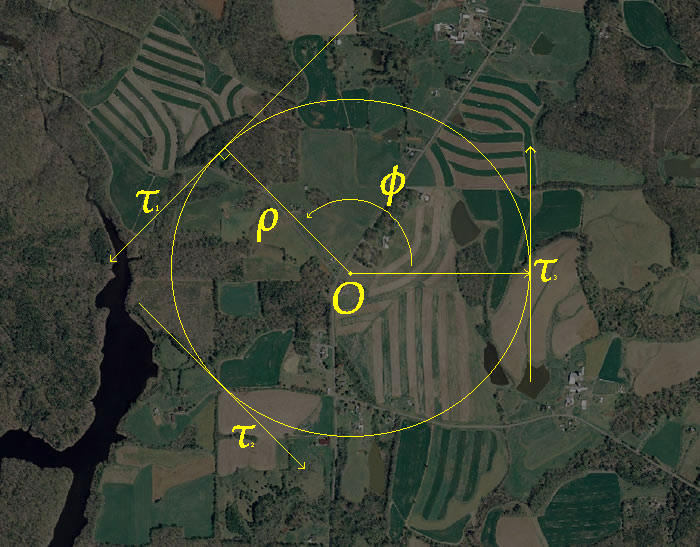
\includegraphics[width=1\textwidth]{images/trazos.png}
    \caption{Parametros de la TT. En la figura se presenta desde el punto de origen $O$, la rotación $\phi$, la distancia desde el origen $\rho$ y el trazo $\tau$ tangente al circulo de radio $\rho$.}
    \label{fig:trazos}
\end{figure}

El modelo también cuenta con 3 parámetros de frecuencia:
\begin{itemize}
    \item $\Delta \rho$: define cada cuántos píxeles se traza una línea. Si $\Delta \rho$ tiene un valor de 1 píxel se trazarán líneas cada píxel de la imagen, con un valor de 2 píxeles, cada 2 píxeles y así sucesivamente.
    \item $\Delta \phi$: determina cada cuántos grados se trazará una línea. Con un $\Delta \phi$ de 1º se trazarán líneas cada grado para un total de 360, con un valor de 90º, cada ángulo recto para un total de 4 líneas.
    \item $\Delta \tau$: fija, sobre la linea $\tau$, cuales píxeles se tomarán en cuenta para el procesamiento. Si $\Delta \tau$ se carga con un valor de 1 píxel, se utilizarán todos los píxeles de la línea, si tiene un valor de 2 píxeles se tomará una muestra cada 2 y así sucesivamente.
\end{itemize}

%%No es buena idea usar etc. 
Los píxeles que son intersecados por estas líneas $\tau$ y que cumplan con el parámetro $\Delta \tau$ serán la entrada para generar la primera representación de $I$, aplicando el funcional T o de trazo. El resultado será un arreglo de dos dimensiones (que puede ser interpretado como una imagen 2D), $I_T$, definida en parámetros de $\phi$ y $\rho$. El siguiente paso es tomar cada columna de $I_t$ y usarlas como entrada para el funcional P o diamétrico. Esto va a generar un arreglo $I_P$, que es una función del parámetro $\phi$. A este arreglo se le aplica el funcional $\Phi$ o de circo, para dar como resultado un sólo número $I_\Phi$ o característica triple. Este proceso se puede ver gráficamente en al figura \ref{fig:TT}.

Ahora bien, se da el caso en que no sólo es un funcional T, sino una serie, que se pueden indizar en una tabla de funcionales T. Esto produciría múltiples $I_T$ que se pueden denominar $I_T^\tau$, donde $\tau$ es el índice del funcional en la tabla de funcionales T. Esto puede ocurrir y es deseable que ocurra con las otras dos funcionales, ya que esto permite la creación de vectores de TF que puede ser más representativos de $I$ que una sola TF.

\begin{figure}[h!]
    \centering
    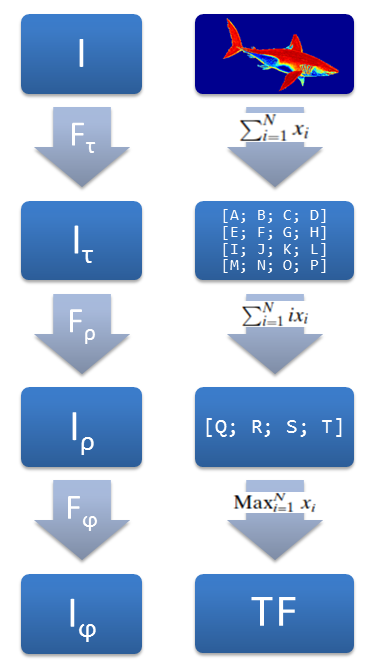
\includegraphics[width=0.5\textwidth]{images/tt.png}
    \caption{Representación gráfica del proceso de la Transformada de Trazo.}
    \label{fig:TT}
\end{figure}

%\bigskip\bigskip
Una vez obtenidas las TF para las imágenes originales, estos vectores de TF deben ser clasificados. Para esto es posible utilizar cualquier clasificador computacional, ya que al obtener una representación vectorial de la imagen se independiza del dominio original.
Clasificadores como redes neuronales artificiales, máquinas de soporte vectorial, agrupaciones, regresiones, entre otros, son todas técnicas válidas para realizar este paso\cite{Ethem2010}.
Como con cualquier clasificador, es necesario hacer una partición del conjunto original de datos; un subconjunto para el entrenamiento y otro para la clasificación.

\subsection{Complejidad de la Transformada de Trazo}

\begin{figure}[H]
    \begin{equation*}
        TF_{N_{\phi} N_{\rho} N_{\tau}} =
        \frac{C_{T}N_{T}n_{\tau}n_{\rho}n_{\phi}}{2} +
        C_{P}N_{P}N_{T}n_{\rho}n_{\phi} +
        C_{\phi}N_{\phi}N_{P}N_{T}n_{\phi}
    \end{equation*}
    \caption{Complejidad del algoritmo de la TT.}
    \label{eq:complejidad}
\end{figure}

La complejidad del algoritmo de la TT está dada por la ecuación de la figura \ref{eq:complejidad}, donde:
\begin{itemize}
    \item $TF_{N_{\phi} N_{\rho} N_{\tau}}$: Total de características triples generadas.
    \item $C_{T}$: cantidad de operaciones para la funcional de trazo hecha sobre cada muestra.
    \item $C_{P}$: cantidad de operaciones para la funcional diamétrica hecha por cada muestra.
    \item $C_{\phi}$: cantidad de operaciones para la funcional de circo hecha por cada muestra.
    \item $N_T$: cantidad de funcionales de trazo.
    \item $N_P$: cantidad de funcionales diamétricas.
    \item $N_\Phi$: cantidad de funcionales de circo.
    \item $n_\tau$: cantidad de muestras del parámetro $\tau$ a lo largo del trazo diagonal más extenso.
    \item $n_\rho$: cantidad de muestras del parámetro $\rho$.
    \item $n_{\phi}$: cantidad de muestras del parámetro $\phi$.
\end{itemize}

El primer término domina considerablemente la complejidad del algoritmo, dado que $n_\tau$, $n_\rho$ y $n_\phi$ son los términos que dependen del tamaño de la entrada mientras que $N_\tau$, $N_\rho$ y $N_\phi$ son los mismos para cualquier tamaño de entrada.

El parámetro de frecuencia $\Delta \tau$ está presente en los tres términos; está representado por $n_\tau$, por lo que es de especial importancia escoger un valor que minimice la cantidad de instrucciones. De igual forma ocurre con $\Delta \rho$ y $\Delta \phi$ pero en menor medida.


\section{Planteamiento del problema}
%Duracion es fea, no hay como saber q un valor para un parametro sea bueno o no, en articulos se han usado diferentes valores, pero no dicen xq. hacer el estudio

Como se mencionó previamente, la TT puede tener un tiempo de ejecución considerable, dependiendo de:
\begin{itemize}
    \item \textbf{Los funcionales utilizados}: existen 31 funcionales asociados a texturas \cite{Petrou2007} que han tenido éxito en sus procesos de clasificación. Son necesarias muchas características para lograr una buena clasificación \cite{Petrou2007}.
    \item \textbf{El tamaño de las imágenes}: las imágenes aéreas utilizadas en el PRIAS tienen tamaños de al menos 5000 $\times$ 5000 pixeles, lo cual es considerable si se toma en cuenta que los estudios anteriores trabajan sobre imágenes mucho más pequeñas \cite{Sayeed2001} \cite{Kadyrov2006} \cite{Albukhanajer2013} \cite{Srisuky2003} \cite{Petrou2007}.
    \item \textbf{Los parámetros de frecuencia (o $\Delta$)}: diferentes estudios muestran que variando estos parámetros es posible obtener buenos resultados \cite{Kadyrov2003} \cite{Petrou2007}, mas no existe un estudio que muestre como afectan estas frecuencias de muestreo a los resultados.
\end{itemize}

Si bien los dos primeros ítemes no se pueden cambiar, el tercero sí. Al no conocerse con exactitud el efecto que pueda tener las variaciones en los parámetros $\delta$ sobre la precisión y el tiempo de ejecución de la TT, se puede estar cayendo en alguna de estas dos situaciones: más trabajo del necesario para lograr una buena clasificación, o bien, es posible que con un poco más de trabajo se pueda lograr una clasificación con una tasa de precisión muy alta.

\section{Hipótesis}

%La Transformada de Trazo puede presentar mejores resultados estadísticamente, tanto en la precisión de la clasificación y/o en el tiempo de respuesta, variando los parámetros de frecuencia.
Basado en la ecuación de complejidad y la revisión del trabajo relacionado, se intuye que los parámetros de frecuencia pueden influir en el tiempo de extracción así como en la calidad de las TF que se generan para la clasificación, lo que lleva a plantear la siguiente hipótesis de investigación:\\

\begin{large}
\textit{La Transformada de Trazo presenta mejores resultados estadísticamente, en precisión de clasificación y en tiempo de extracción de características, al variar los parámetros de frecuencia, el tipo de clasificador y el tipo de cobertura.}
\end{large}

  
\section{Trabajo relacionado}
% articulos donde se ha planeatedo uso distinto de los parametros

Desde la elaboración conceptual de la TT en el 2001 \cite{Kadyrov2001}, esta ha producido varias publicaciones de casos de estudio en diferentes áreas.
%% uso historico o previo

La TT es una generalización de la transformada de Radon \cite{Ginkel2004} \cite{Kadyrov2003} en la que se calcula como funcional de trazo la integral del mismo trazo. Este método ha sido utilizado en tomografía e imagenología médica \cite{Tutorial2008}.

Previo a la publicación de la TT, ya se manejaba la idea de extraer características invariantes de imágenes para la clasificación. En \cite{Sayeed2001}, se realizó una extracción de características para determinar si un paciente padecía de Alzheimer. Dicho estudio tuvo una precisión del 88\% al clasificar dichas imágenes.
%% exitos en clasificacion


Es posible identificar huellas de insectos utilizando la TT junto con otros métodos para la segmentación de imágenes. En \cite{Bok2008} se muestra una mejora de entre 7\% y 63\% en comparación con el método convencional \cite{Shin2007}.

La TT se puede combinar con otros métodos para extraer características robustas. La combinación con algoritmos evolutivos mostró que da buenos resultados al clasificar TF \cite{Albukhanajer2013}.

Las características de invarianza o sensibilidad de las TF se pueden comparar en \cite{Turan2005}. Aquí una serie de imágenes de referencia se compara con imágenes que han sido sujetas a transformaciones afines: rotación, desplazamiento y escalamiento. El estudio concluyó que la TT, usando la combinación de funcionales correctas tiene una precisión de entre 98\% y 100\%.

La TT se puede utilizar para clasificar o reconocer imágenes más complejas como rostros. En \cite{Srisuky2003} se compara el método Eigenfaces\cite{Zhang1997} con una modificación de la TT llamada: ``Masked Trace Transform'' + ``Weighted Trace Transform''. El método basado en la TT tuvo mejor desempeño en modificaciones como rotación, escalamiento y cambio en la expresión facial.
%% exitos en clasificacion con texturas

%% uso de distintos deltas
La variación de parámetros para producir las TF no es muy común y se utiliza una configuración estándar. Aun así, hay varios estudios donde se obtuvieron buenos resultados. En \cite{Kadyrov2003} se realizaron experimentos para crear firmas únicas para imágenes utilizando características extraídas con la TT. Aquí, los parámetros para $\Delta \rho$, $\Delta \tau$ y $\Delta \phi$ fueron respectivamente, 2 píxeles, 2 píxeles  y 3º. El estudio reveló que las TF tienen un desempeño similar a las características extraídas con otros métodos, pero las primeras son más robustas y resistentes al cambio.

En \cite{Petrou2007} se comparan las características extraídas por métodos automáticos como la TT contra otros más rígidos como con el uso de matrices de co-ocurrencia, con base a la forma en como las personas interpretan las texturas. En general, las características extraídas con la TT se puede modelar de manera semejante a la forma en que los humanos perciben las texturas. En los experimentos realizados en este estudio, se utilizó, a diferencia de los experimentos previos, un $\Delta \rho$ de 2.




